\documentclass[a4paper,11pt]{article}

\usepackage[T1]{fontenc}
\usepackage[utf8]{inputenc}
\usepackage{tabularx}
\usepackage{multirow,array}
\usepackage{amsmath}
\usepackage{amssymb}
\usepackage{mathabx}
\usepackage{tikz}
\usepackage{fancyhdr}
\usepackage{lastpage}
\usepackage{hyperref}

\usepackage{graphicx}
\graphicspath{ {./} }

\usepackage{geometry}
\geometry{left=25mm,right=25mm,bindingoffset=10mm, top=22mm,bottom=30mm, footskip=10mm}
\setlength{\parindent}{0pt}
\setlength{\headsep}{0.5in}




\linespread{1.3}

\pagestyle{fancy}
\fancyhf{}
\rhead{
  ECON 4673 Assignment \#1 \\
  Albert Lockett, 3254354
}
\rfoot{Page \thepage / \pageref{LastPage}\\}


\begin{document}
\title{ECON 4673 Assignment \#1}
\author{
  Albert Lockett \\ 
  3254354, 
  \href{mailto:me@somewhere.com}{\texttt{k44if@unb.ca}}
  }
\date{01/22/2021}

\maketitle

\section*{Problem 1}

\begin{table}[htbp]
  \begin{tabularx}{\textwidth}{lXc}
    {\bf \#} & {\bf Statement} & {\bf True/False}  \\ \hline
    1 & Every finite normal-form game has a pure strategy Nash equilibrium.     & \texttt{false}  \\ 
    2 & Every dominant strategy equilibrium is also a Nash equilibrium.         & \texttt{true}  \\
    3 & It is possible that there might exist some pure strategy Nash 
        equilibria which did not survive the iterated elimination of strictly 
        dominated strategies.                                                   & \texttt{true} \\
    4 & A strictly dominated strategy can also be a Nash equilibrium.           & \texttt{false}  \\
    5 & Every Nash equilibrium is also a dominant strategy equilibrium.         & \texttt{false}  \\
    5 & Every rationalizable strategy profile is also a Nash equilibrium.       & \texttt{false}  \\
  \end{tabularx}
  
\end{table}


\section*{Problem 2}

\begin{table}[htbp]
  \setlength{\extrarowheight}{2pt}
  \begin{tabular}{*{4}{c|}}
    \multicolumn{2}{c}{} & \multicolumn{2}{c}{Player $2$}\\\cline{3-4}
    \multicolumn{1}{c}{}       &     &   $C$ &   $D$   \\\cline{2-4}
    \multirow{2}*{Player $1$}  & $A$ & $1,1$ & $2,0$ \\\cline{2-4}
                               & $B$ & $0,2$ & $x,y$ \\\cline{2-4}
  \end{tabular}
\end{table}

\subsection*{2.1)}

Thse values will lead to a dominant strategy equillibrium of $(A, C)$:

\[ x < 2 \]
\[ y < 2 \]

What follows is justification for the solution ... \newline

Player 1's strategy $A$ will be dominant if $A$ has a greater payoff than strategy $B$ for all strategies of Player 2.
\[ u_1(A, s_2) > u_1(B, s_2) \hspace{2mm} \forall \hspace{2mm} s_2 \in S_2 = \{ C, D, \sigma_2 \} \]
where $\sigma_2$ is a mixed strategy with probbility $0 < p < 1$ that $s_2 = D$.\newline 

When $s_2 = C$, it is given that $s_1 = A$ has a higher payoff than $s_2 = B$.
\[ u_1(A, C) = 1 > u_1(B, C) = 0 \]

To satisfy the condition of dominance same must be true for $s_2 = D$:
\[ u_1(A, D) = 2 > u_1(B, D) = x \]
\[ x < 2 \]

For the mixed strategy case:

\[ u_1(A, \sigma_2) = u_1(A, C)(1 - p) + u_1(A, D)p = 1(1 - p) + 2p = 1 + p \]
\[ u_1(B, \sigma_2) = u_1(B, C)(1 - p) + u_1(B, D)p = 0(1 - p) + xp = xp \]

To satisfy the dominance condition:
\[ u_1(A, \sigma_2) > u_1(B, \sigma_2)\]
\[ 1 + p > xp \hspace{2mm} \]

The relationship is satisfied for $0 < p < 1$ if $x < 2$, which can be seen graphically:

\begin{center}
  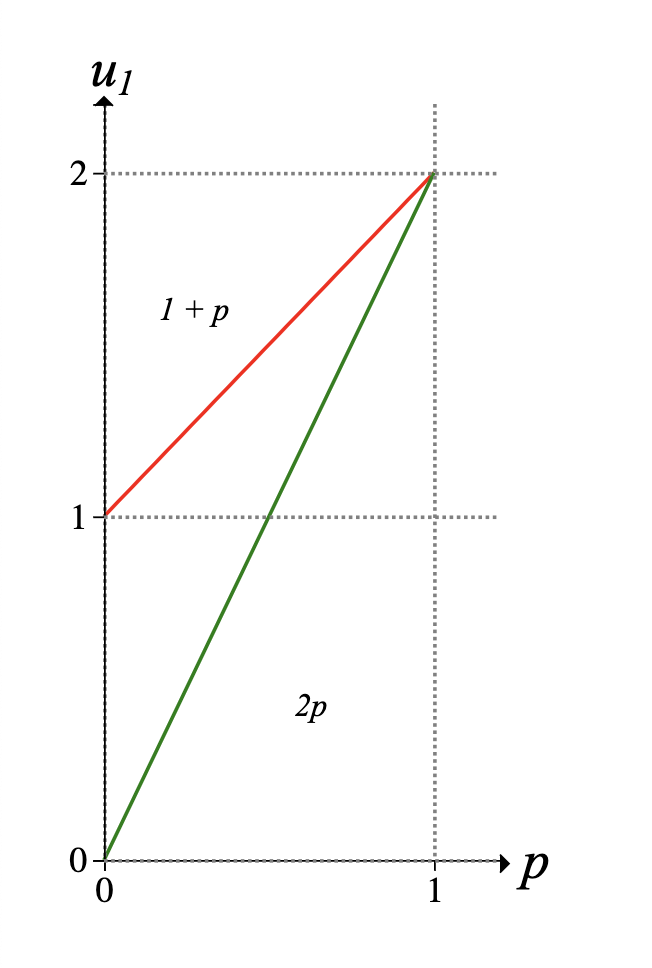
\includegraphics[scale=0.5]{prob_2_1_fig1.png}
\end{center}

The same analysis for player 2:

\[ u_2(s1, C) > u_2(s1, D) \hspace{2mm} \forall \hspace{2mm} s_1 \in S_1 = \{ A, B, \sigma_1 \} \]

\begin{center}
($\sigma_1$ is a mixed strategy with probbility $0 < p < 1$ that $s_1 = B$)
\end{center}
\[ u_2(A, C) = 1 > u_2(A, D) = 0 \]

\[ u_2(B, C) = 2 > u_2(B, D) = y \]
\[ y < 2 \]

\[ u_2(\sigma_1, C) =  1 + p \]
\[ u_2(\sigma_1, D) = yp \]

\[ u_2(\sigma_1, C) > u_2(\sigma_1, D) \]
\[ 1 + p > yp \hspace{2mm},\hspace{2mm} 0 < p < 1 \implies y < 2 \]



\subsection*{2.2)}

These values will make this game into a \textit{Prisoner's Dilemna}:

\[ 1 < x < 2 \]
\[ 1 < y < 2 \]

In a \textit{Prisoner's Dilemna} there are three scenarios that can occur:\\

\textit{Scenario 1}: Both criminals defect\\

The authorities offer each of the criminals the opportunity to testify on the other in exchange for a reduced sentence.
In this scenario, both criminals accept the offer and testify against the other (strategy $D$).
They receive a payoff value $x_1$ representing the reduced sentence.
\[ u_1(D,D) = u_2(D, D) = x_1 \]

\textit{Scenario 2}: One criminal cooperates \& the other defects\\

Criminal $i$ decides to testify against the other ($s_i = D$) and is freed, which means this criminal's payoff $x_{2i}$ is higher
than in scenario 1.The other criminal $-i$ does not testify ($s_{-i} = C$), which means they get the full sentence 
for the crime so their payoff $x_{2ii}$ is lower than the payoff from scenario 1.

\[ u_i(C,D) = x_{2i} > x_1 \]
\[ u_{-i}(C,D) = x_{2ii} < x_1 \]

\vspace{12px}
\textit{Scenario 3: Criminals Cooperation}\\

Each criminal decides not to testify on the other so the authorities are only able to convict them of a minor
offense. The sentence is less harsh than the sentence for the main crime, which means the payoff value $x_3$ is higher
than in scenario 1, but not as high as the case where the criminal goes free.

\[ x_1 < u_1(C,C) = u_2(C, C) = x_3 < x_{2i} \]

The prisoner's dilemna in normal form:
\begin{table}[htbp]
  \setlength{\extrarowheight}{2pt}
  \begin{center}
  \begin{tabular}{*{4}{c|}}
    \multicolumn{2}{c}{} & \multicolumn{2}{c}{Criminal $1$}\\\cline{3-4}
    \multicolumn{1}{c}{}         &     &   $D$              &   $C$               \\\cline{2-4}
    \multirow{2}*{Criminal $1$}  & $D$ & $x_1,x_1$        & $x_{2i},x_{2ii}$  \\\cline{2-4}
                                 & $C$ & $x_{2i},x_{2ii}$ & $x_3,x_3$         \\\cline{2-4}
  \end{tabular}\\
  \[ x_{2ii} < x_1 < x_3 < x_{2ii} \]
  \end{center}
\end{table}


Substituting the payoff from the game in the problem:

\[ x_1 = 1, \hspace{2mm} x_{2i} = 2, \hspace{2mm} x_{2ii} = 0\]

\begin{table}[htbp]
  \setlength{\extrarowheight}{2pt}
  \begin{center}
  \begin{tabular}{*{4}{c|}}
    \multicolumn{2}{c}{} & \multicolumn{2}{c}{Criminal $1$}\\\cline{3-4}
    \multicolumn{1}{c}{}         &     &   $D$   &   $C$   \\\cline{2-4}
    \multirow{2}*{Criminal $1$}  & $D$ & $1,1$ & $2,0$ \\\cline{2-4}
                                 & $C$ & $0,2$ & $x_3,x_3$ \\\cline{2-4}
  \end{tabular}\\
  \[ 0 < 1 < x_3 < 2 \]
  \end{center}
\end{table}

\clearpage
\section*{Problem 3}

\begin{table}[!htbp]
  \setlength{\extrarowheight}{2pt}
  \begin{center}
  \begin{tabular}{*{4}{c|}}
    \multicolumn{2}{c}{} & \multicolumn{2}{c}{Player $2$}\\\cline{3-4}
    \multicolumn{1}{c}{}       &     &   $X$ &   $Y$   \\\cline{2-4}
    \multirow{2}*{Player $1$}  & $A$ & $3,3$ & $0,1$ \\\cline{2-4}
                               & $B$ & $5,5$ & $2,2$ \\\cline{2-4}
  \end{tabular}\\
  \end{center}
\end{table}

\subsection*{3.1)}

The only pure strategy Nash equillibrium is $(B,X)$.\\

The condition for Nash equilibrium
\[ s_i \in BR_i(s_{-1}) \hspace{2mm} \forall \hspace{2mm} i \]

Strategy $Y$ is dominated by $X$, which means $s_2 = X$ is always best response\\
\[ BR_2(s_1) = \{X\} \hspace{2mm} \forall \hspace{2mm} S_1 \]

$s_1 = B$ is the best response to $X$
\[ BR_1(X) = B \]

\subsection*{3.2)}

Let $\sigma_1$ be a mixed strategy with probability $0 < p < 1$ that $s_1 = A$

Let $\sigma_2$ be a mixed strategy with probability $0 < q < 1$ that $s_2 = X$\\

A Nash equillibrium will exist $p = 0$ and $q = 1$ which results in the strategy profile $(B,X)$\\

Player 1's expected payoff
\[ v_1(\sigma_1, \sigma_2) = \sum_{(s_1, s_2)} u_2(s_1, s_2) P(s = (s_1, s_2)), \hspace{2mm} (s_1, s_2) \in S_1 \bigtimes S_2 \]
\[ = u_1(A,X)pq + u_1(A,Y)p(1 - q) + u_1(B,X)(1 - p)q + u_1(B,Y)(1 - p)(1 - q)\] 
\[ = 3pq + 0p(1 - q) + 5(1 - p)q + 2(1 - p)(1 - q) \] 
\[ =  3q  - 2p + 2 \]

It is strictly decreasing with $p$

\[ \frac{\partial}{\partial p} v_1(\sigma_1, \sigma_2) = -2 \]

$v_1(\sigma_1, \sigma_2)$ is maximized when $p$ is minimized, so for any given $q$, $p$ = 0 is best.
\[ BR_1(\sigma_2) = B,\hspace{2mm} 0 < q < 1 \]

\vspace{12px}

The same analysis to determine player 2's expected payoff
\[ v_2(\sigma_1, \sigma_2) = \sum_{(s_1, s_2)} u_2(s_1, s_2) P(s = (s_1, s_2)), \hspace{2mm} (s_1, s_2) \in S_1 \bigtimes S_2 \]
\[ = u_2(A,X)pq + u_2(A,Y)p(1 - q) + u_2(B,X)(1 - p)q + u_2(B,Y)(1 - p)(1 - q)\] 
\[ = 3pq + 1p(1 - q) + 5(1 - p)q + 2(1 - p)(1 - q) \] 
\[ =  -pq -p + 3q + 2 \]

It is strictly increasing with q over the interval $0 < p < 1$
\[ \frac{\partial}{\partial p} v_2(\sigma_1, \sigma_2) = -p + 3 > 0, \hspace{2mm} 0 < p < 1 \]

Player 2 will maximize the payoff with the largest possible value $q = 1$
\[ BR_2(\sigma_1) = X,\hspace{2mm} 0 < p < 1 \]


\section*{Problem 4}

\begin{table}[htbp]
  \setlength{\extrarowheight}{2pt}
  \begin{center}
  \begin{tabular}{*{5}{c|}}
    \multicolumn{2}{c}{} & \multicolumn{2}{c}{Player $2$}\\\cline{3-5}
    \multicolumn{1}{c}{}       &     &   $L$ &   $M$ & $R$ \\\cline{2-5}
    \multirow{2}*{Player $1$}  & $T$ & $1,-1$ & $5,0$ & $0,0$ \\\cline{2-5}
                               & $C$ & $0,5$  & $4,4$ & $0,0$ \\\cline{2-5}
                               & $B$ & $0,0$  & $0,0$ & $3,3$ \\\cline{2-5}
  \end{tabular}\\
  \end{center}
\end{table}

\subsection*{4.1)}

The relationalizable strategies are $\{M, R\} \bigtimes \{T, B\}$.
Rationalizable strategies are those which can survive the process of iterated dominance.
Strategies $C$ and $L$ can be dominated.
\\

Strategy $C$ can be dominated by a mixed strategy $\sigma_1$ with of playing $T$, $C$ and $B$ 
of
\[4/5 < p_T < 1 \]
\[p_C = 0 \] 
\[p_B  = 1 - p_T \]

For example $p_T =$ 0.85 $\implies$ $p_B =$ 0.15
\[ u_1(\sigma_1, L) = 0.85(1) + 0 + 0 = 0.85 > u_1(C, L) = 0\] 
\[ u_1(\sigma_1, M) = 0.85(5) + 0 + 0 = 4.25 > u_1(C, M) = 4\]
\[ u_1(\sigma_1, R) = 0 + 0 + .15(3) = 0.45 > u_1(C, R) = 0\]

\vspace{1cm}
The game with $C$ removed:
\begin{table}[htbp]
  \setlength{\extrarowheight}{2pt}
  \begin{center}
  \begin{tabular}{*{5}{c|}}
    \multicolumn{2}{c}{} & \multicolumn{2}{c}{Player $2$}\\\cline{3-5}
    \multicolumn{1}{c}{}       &     &   $L$ &   $M$ & $R$ \\\cline{2-5}
    \multirow{2}*{Player $1$}  & $T$ & $1,-1$ & $5,0$ & $0,0$ \\\cline{2-5}
                               & $B$ & $0,0$  & $0,0$ & $3,3$ \\\cline{2-5}
  \end{tabular}\\
  \end{center}
\end{table}

In the new game, strategy $L$ is dominated by a mixed strategy $\sigma_2$ of playing $L$, $M$ and $R$ of
\[ p_L = 0 \]
\[ 0 < p_M < p_R < 1 \]

For example $p_M =$ 0.5 $\implies$ $p_B =$ 0.5
\[ u_2(T, \sigma_2) = 0 + 0.5(5) + 0 = 0.25 > u_2(T, L) = -1 \]
\[ u_2(B, \sigma_2) = 0 + 0 + 3(0.5) = 1.5 > u_2(B, L) = 0 \]

\vspace{1cm}
The resulting game with $L$ removed:
\begin{table}[htbp]
  \setlength{\extrarowheight}{2pt}
  \begin{center}
  \begin{tabular}{*{4}{c|}}
    \multicolumn{2}{c}{} & \multicolumn{2}{c}{Player $2$}\\\cline{3-4}
    \multicolumn{1}{c}{}       &     &   $M$ & $R$ \\\cline{2-4}
    \multirow{2}*{Player $1$}  & $T$ & $5,0$ & $0,0$ \\\cline{2-4}
                               & $B$ & $0,0$ & $3,3$ \\\cline{2-4}
  \end{tabular}\\
  \end{center}
\end{table}

There are no more dominated strategies.

\vspace{2cm} 
\subsection*{4.2)}

There are two Nash equilibria $(T,M)$ and $(B, R)$.\\

The condition for Nash equilibrium
\[ u_i(s_i, s_{-1}) > u_i(s'_i, s_{-1}) \hspace{2mm} \forall \hspace{2mm} i,\hspace{2mm} s'_i \in S_i \]

(T,M) is a Nash equillibrium but (T,R) is not:
\[ u_1(T, M) = 5 > u_1(T, R) = 0 \]
\[ u_2(T, M) = 0 \ge u_2(T, R) = 0 \]


(B,R) is a Nash equillibrium but (B,M) is not:
\[ u_1(B, R) = 3 > u_1(T, R) = 0 \]
\[ u_2(B, R) = 3 > u_2(B, M) = 0 \]

\subsection*{4.3)}

There is not a dominant strategy equilibrium for the game.

\end{document}






